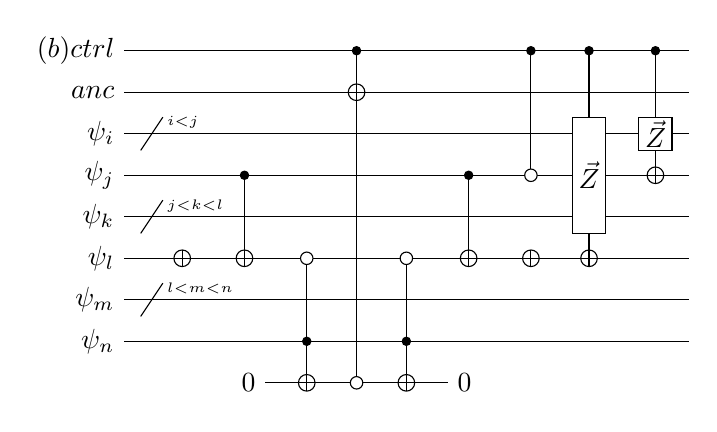
\begin{tikzpicture}[scale=1.000000,x=1pt,y=1pt]
\filldraw[color=white] (0.000000, -7.500000) rectangle (204.000000, 127.500000);
% Drawing wires
% Line 1: c W \text{(b) }ctrl
\draw[color=black] (0.000000,120.000000) -- (204.000000,120.000000);
\draw[color=black] (0.000000,120.000000) node[left] {$\text{(b) }ctrl$};
% Line 2: a W anc
\draw[color=black] (0.000000,105.000000) -- (204.000000,105.000000);
\draw[color=black] (0.000000,105.000000) node[left] {$anc$};
% Line 3: i W \psi_i
\draw[color=black] (0.000000,90.000000) -- (204.000000,90.000000);
\draw[color=black] (0.000000,90.000000) node[left] {$\psi_i$};
% Line 4: j W \psi_j
\draw[color=black] (0.000000,75.000000) -- (204.000000,75.000000);
\draw[color=black] (0.000000,75.000000) node[left] {$\psi_j$};
% Line 5: k W \psi_k
\draw[color=black] (0.000000,60.000000) -- (204.000000,60.000000);
\draw[color=black] (0.000000,60.000000) node[left] {$\psi_k$};
% Line 6: l W \psi_l
\draw[color=black] (0.000000,45.000000) -- (204.000000,45.000000);
\draw[color=black] (0.000000,45.000000) node[left] {$\psi_l$};
% Line 7: m W \psi_m
\draw[color=black] (0.000000,30.000000) -- (204.000000,30.000000);
\draw[color=black] (0.000000,30.000000) node[left] {$\psi_m$};
% Line 8: n W \psi_n
\draw[color=black] (0.000000,15.000000) -- (204.000000,15.000000);
\draw[color=black] (0.000000,15.000000) node[left] {$\psi_n$};
% Line 9: clean W 0 0
\draw[color=black] (43.500000,0.000000) -- (124.500000,0.000000);
% Done with wires; drawing gates
% Line 11: i / ^{i<j}
\draw (6.000000, 84.000000) -- (14.000000, 96.000000);
\draw (12.000000, 93.000000) node[right] {$\scriptstyle{^{i<j}}$};
% Line 12: k / ^{j<k<l}
\draw (6.000000, 54.000000) -- (14.000000, 66.000000);
\draw (12.000000, 63.000000) node[right] {$\scriptstyle{^{j<k<l}}$};
% Line 13: m / ^{l<m<n}
\draw (6.000000, 24.000000) -- (14.000000, 36.000000);
\draw (12.000000, 33.000000) node[right] {$\scriptstyle{^{l<m<n}}$};
% Line 14: c a i j k l m n clean LABEL width=-20
% Line 16: +l
\begin{scope}
\draw[fill=white] (21.000000, 45.000000) circle(3.000000pt);
\clip (21.000000, 45.000000) circle(3.000000pt);
\draw (18.000000, 45.000000) -- (24.000000, 45.000000);
\draw (21.000000, 42.000000) -- (21.000000, 48.000000);
\end{scope}
% Line 17: j +l
\draw (43.500000,75.000000) -- (43.500000,45.000000);
\filldraw (43.500000, 75.000000) circle(1.500000pt);
\begin{scope}
\draw[fill=white] (43.500000, 45.000000) circle(3.000000pt);
\clip (43.500000, 45.000000) circle(3.000000pt);
\draw (40.500000, 45.000000) -- (46.500000, 45.000000);
\draw (43.500000, 42.000000) -- (43.500000, 48.000000);
\end{scope}
% Line 18: clean START
\draw[color=black] (51.000000,0.000000) node[fill=white,left,minimum height=15.000000pt,minimum width=15.000000pt,inner sep=0pt] {\phantom{$0$}};
\draw[color=black] (51.000000,0.000000) node[left] {$0$};
% Line 19: n -l +clean
\draw (66.000000,45.000000) -- (66.000000,0.000000);
\filldraw (66.000000, 15.000000) circle(1.500000pt);
\draw[fill=white] (66.000000, 45.000000) circle(2.250000pt);
\begin{scope}
\draw[fill=white] (66.000000, 0.000000) circle(3.000000pt);
\clip (66.000000, 0.000000) circle(3.000000pt);
\draw (63.000000, 0.000000) -- (69.000000, 0.000000);
\draw (66.000000, -3.000000) -- (66.000000, 3.000000);
\end{scope}
% Line 20: c -clean +a
\draw (84.000000,120.000000) -- (84.000000,0.000000);
\filldraw (84.000000, 120.000000) circle(1.500000pt);
\draw[fill=white] (84.000000, 0.000000) circle(2.250000pt);
\begin{scope}
\draw[fill=white] (84.000000, 105.000000) circle(3.000000pt);
\clip (84.000000, 105.000000) circle(3.000000pt);
\draw (81.000000, 105.000000) -- (87.000000, 105.000000);
\draw (84.000000, 102.000000) -- (84.000000, 108.000000);
\end{scope}
% Line 21: n -l +clean
\draw (102.000000,45.000000) -- (102.000000,0.000000);
\filldraw (102.000000, 15.000000) circle(1.500000pt);
\draw[fill=white] (102.000000, 45.000000) circle(2.250000pt);
\begin{scope}
\draw[fill=white] (102.000000, 0.000000) circle(3.000000pt);
\clip (102.000000, 0.000000) circle(3.000000pt);
\draw (99.000000, 0.000000) -- (105.000000, 0.000000);
\draw (102.000000, -3.000000) -- (102.000000, 3.000000);
\end{scope}
% Line 22: clean END
\draw[color=black] (117.000000,0.000000) node[fill=white,right,minimum height=15.000000pt,minimum width=15.000000pt,inner sep=0pt] {\phantom{$0$}};
\draw[color=black] (117.000000,0.000000) node[right] {$0$};
% Line 23: j +l
\draw (124.500000,75.000000) -- (124.500000,45.000000);
\filldraw (124.500000, 75.000000) circle(1.500000pt);
\begin{scope}
\draw[fill=white] (124.500000, 45.000000) circle(3.000000pt);
\clip (124.500000, 45.000000) circle(3.000000pt);
\draw (121.500000, 45.000000) -- (127.500000, 45.000000);
\draw (124.500000, 42.000000) -- (124.500000, 48.000000);
\end{scope}
% Line 24: +l
\begin{scope}
\draw[fill=white] (147.000000, 45.000000) circle(3.000000pt);
\clip (147.000000, 45.000000) circle(3.000000pt);
\draw (144.000000, 45.000000) -- (150.000000, 45.000000);
\draw (147.000000, 42.000000) -- (147.000000, 48.000000);
\end{scope}
% Line 26: c -j
\draw (147.000000,120.000000) -- (147.000000,75.000000);
\filldraw (147.000000, 120.000000) circle(1.500000pt);
\draw[fill=white] (147.000000, 75.000000) circle(2.250000pt);
% Line 28: i j k G $\vec{Z}$ c +l
\draw (168.000000,120.000000) -- (168.000000,45.000000);
\begin{scope}
\draw[fill=white] (168.000000, 75.000000) +(-45.000000:8.485281pt and 29.698485pt) -- +(45.000000:8.485281pt and 29.698485pt) -- +(135.000000:8.485281pt and 29.698485pt) -- +(225.000000:8.485281pt and 29.698485pt) -- cycle;
\clip (168.000000, 75.000000) +(-45.000000:8.485281pt and 29.698485pt) -- +(45.000000:8.485281pt and 29.698485pt) -- +(135.000000:8.485281pt and 29.698485pt) -- +(225.000000:8.485281pt and 29.698485pt) -- cycle;
\draw (168.000000, 75.000000) node {$\vec{Z}$};
\end{scope}
\filldraw (168.000000, 120.000000) circle(1.500000pt);
\begin{scope}
\draw[fill=white] (168.000000, 45.000000) circle(3.000000pt);
\clip (168.000000, 45.000000) circle(3.000000pt);
\draw (165.000000, 45.000000) -- (171.000000, 45.000000);
\draw (168.000000, 42.000000) -- (168.000000, 48.000000);
\end{scope}
% Line 29: i G $\vec{Z}$ c +j
\draw (192.000000,120.000000) -- (192.000000,75.000000);
\begin{scope}
\draw[fill=white] (192.000000, 90.000000) +(-45.000000:8.485281pt and 8.485281pt) -- +(45.000000:8.485281pt and 8.485281pt) -- +(135.000000:8.485281pt and 8.485281pt) -- +(225.000000:8.485281pt and 8.485281pt) -- cycle;
\clip (192.000000, 90.000000) +(-45.000000:8.485281pt and 8.485281pt) -- +(45.000000:8.485281pt and 8.485281pt) -- +(135.000000:8.485281pt and 8.485281pt) -- +(225.000000:8.485281pt and 8.485281pt) -- cycle;
\draw (192.000000, 90.000000) node {$\vec{Z}$};
\end{scope}
\filldraw (192.000000, 120.000000) circle(1.500000pt);
\begin{scope}
\draw[fill=white] (192.000000, 75.000000) circle(3.000000pt);
\clip (192.000000, 75.000000) circle(3.000000pt);
\draw (189.000000, 75.000000) -- (195.000000, 75.000000);
\draw (192.000000, 72.000000) -- (192.000000, 78.000000);
\end{scope}
% Done with gates; drawing ending labels
% Done with ending labels; drawing cut lines and comments
% Done with comments
\end{tikzpicture}
